\newpage

\refstepcounter{section}
%Add Image
\vspace*{-40mm} %Make image have no top margin
\begin{tikzpicture}
\node[inner sep=0pt] (x) at (0,0)
    {\hspace{-87mm}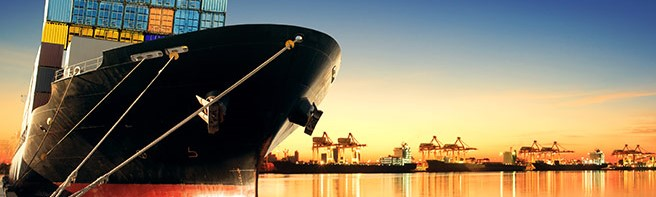
\includegraphics[width=\paperwidth]{sectionimage1.jpg}};
\node[text width=10in] (Z) at (0,-1) {\color{white}\headingfont\Large\bfseries\uppercase{\hspace{-0.7cm}\thesection\hspace{0.5cm}Stakeholder Analysis}};
\end{tikzpicture}
%Modify TOC
\addcontentsline{toc}{section}{\protect\numberline{\thesection}Stakeholder Analysis}
  \sectionmark{Stakeholder Analysis}
\vspace{-5mm}

%Content
% \section{Stakeholder Analysis}
    % \setlength{\columnsep}{0.5cm}
\begin{multicols}{2}
\subsection*{Auckland Council \& Residents} %of Auckland City, Whangarei, Tauranga}
    \textbf{The Auckland Council organisation as a whole is responsible for operation and service delivery, advising the governing body and local boards and carrying out their decisions. They represent the local Auckland residents. Residents include those who live in  the city and downtown areas that may be directly affected by construction on the waterfront. They are the consumers of shipped products}
    \\Auckland Council currently holds 100\% ownership of the Port of Auckland, receiving a net profit after tax as reported in 2017 of \$60.3 million per year. The Auckland Council is likely to be resistive to a relocation of the port outside of Auckland as removing freight removes a major source of revenue. Auckland already supports a population of 1.65 million and this number continues to rise at a rate of 1.9\% per annum. This growing population has growing demand and in turn, a larger volume of freight is needed to support this.
\subsection*{Central Government}
    \textbf{The New Zealand Central Government contains working groups that investigate the feasibility of projects and report directly to the Cabinet Office, influencing government decision making. They are interested in the continued economic growth of the country and will take into consideration factors in New Zealand’s revenue that influence this, namely tourism.}
    \\Alongside executive decision making power, the Central Government is assumed to provide significant funding and is likely to be supportive of the project if it is perceived to add value to the country and the government reputation. For tourism, Cruise ships docking in the PoA currently contribute an estimated \$204 million to the \$7.4 billion Auckland visitor economy. It is predicted by 2030 that this will rise to a \$470 million contribution. This increased tourism income will require more docking capacity for these cruise ships and less freight ship congestion in Auckland.
\subsection*{Transport Agencies}
    \textbf{Local government controlled agencies are responsible for developing possible transport solutions around New Zealand. Within this, KiwiRail is the largest rail transport operator in New Zealand. They are responsible for all rail operations in New Zealand. Their main aim will be to ensure the roads and/or railways are fit for purpose.}  
    \\ Responsible for any new roading and/or rail built in the case of a relocated port. Transport routes and frequency will have to change to accommodate for redistribution of freight. Transport agencies will not be significant contributors, however will be supportive if it does require any developments of the current road network.
\subsection*{Other City Councils}
    \textbf{Tauranga City Council, Northland City Council, and Whangarei District Council will meet the requirements of the locals by providing substantial development within their respective areas. }
    \\With regards to relocation of the Auckland port, other city councils will be significantly important and supportive. These councils would want to develop current infrastructure of the ports to compensate for the immediate future. These councils represent both the residents of their regions and their respective ports. This will provide more job opportunities for the different regions and with this, will be able to generate additional revenue. These job opportunities and revenue help to provide the growth needed to further develop any necessities required by the councils.
\subsection*{Port of Auckland Users}
    \textbf{Port Workers encompass everyone directly affected by the final solution. This includes any shipping company in Auckland and any current workers as they have to change their destination if there is reallocation. Moving and distributing freight via the Auckland Port will also be considered as Port users.}
    \\The Port of Auckland currently employs 500 direct jobs and they support approximately 187,000 jobs that facilitate the port proceedings. Reallocation of the Auckland port will result in redundancy of employees and a change in freight destination for shipping companies.  Some workers will be required to relocate with many unable to move. This will come at a great personal/financial cost for many of the workers.
\subsection*{Investors}
    \textbf{Investors provide feasibility for all projects around New Zealand. To cope with relocation of the port, they will be of high importance and will be supportive provided the relocated port can provide with a greater return of their investments.}
    \\The investors are companies, individuals, groups or organisations assumed to be providing funds for the project. They will expect a substantial return on investments.
    
% \subsection{Stakeholder 4}
% \lipsum[1-2]
% \subsection{Stakeholder 5}
% \lipsum[1]
\end{multicols}

\begin{wrapfigure}{l}{\linewidth}
\centering

\includegraphics[width=0.7\textwidth]{StakeholderMatrix.png}
\centering
\caption{Stakeholder Analysis Matrix}
\end{wrapfigure}


%Restore geometry 
% \restoregeometry
\clearpage